%% pie_charts.tex
%% Author: Leighton Pritchard
%% Copyright: James Hutton Institute
%% What does the evidence say about pie charts?

% PEOPLE HATE PIE CHARTS
\begin{frame}
  \frametitle{People hate pie charts}
    \begin{scriptsize}    
    \href{http://www.storytellingwithdata.com/blog/2011/07/death-to-pie-charts}{http://www.storytellingwithdata.com/blog/2011/07/death-to-pie-charts} \\
    \begin{alertblock}{especially Edward Tufte}
    A table is nearly always better than a dumb pie chart; the only worse design than a pie chart is several of them[...] pie charts should never be used. - \textit{"The Visual Display of Quantitative Information"}
    \end{alertblock}
    \end{scriptsize}
    \begin{center}
      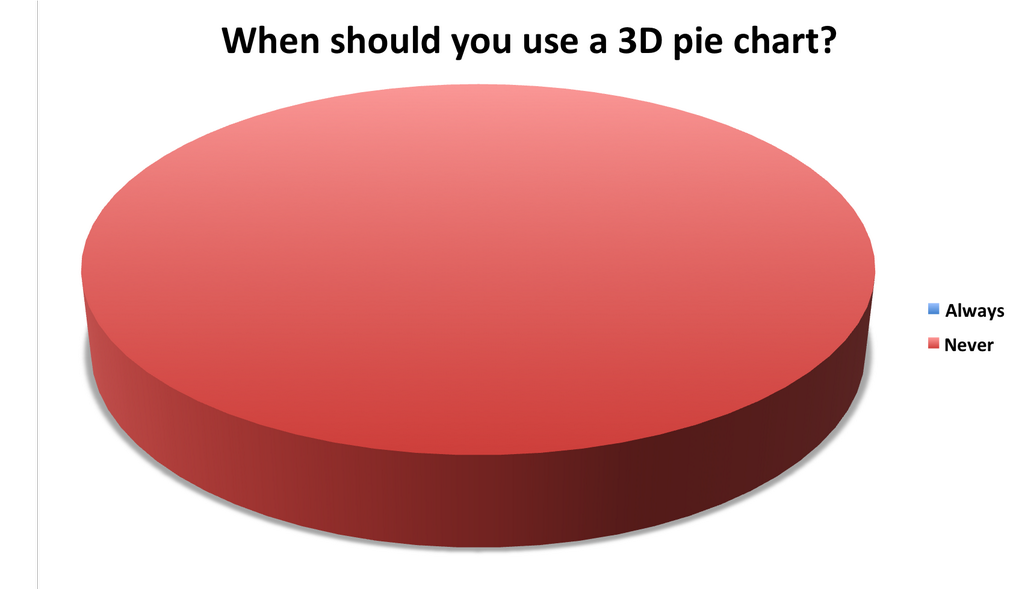
\includegraphics[height=0.5\textheight]{images/3d_pie_chart}
      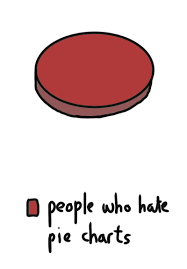
\includegraphics[height=0.5\textheight]{images/people_hate_pie_charts}
    \end{center}
\end{frame}

% BUT THEY HAVE USES
\begin{frame}
  \frametitle{"E pur si muove$\ldots$"
  \footnote{\tiny{\href{http://www.jstor.org/stable/2277140}{Eells (1926) \textit{J Am. Stat. Ass.}}}}
  \footnote{\tiny{\href{http://www.jstor.org/stable/2289447}{Simkin \& Hastie (1987) \textit{J Am. Stat. Ass.}}}}
  }
  \begin{scriptsize}
    \begin{alertblock}{For proportions of a whole:}
      \begin{itemize}
        \item Pie charts read as accurately as bar charts
        \item As number of components in the chart increases, bars are less efficient than pie charts
      \end{itemize}
    \end{alertblock}
  \end{scriptsize}
  \begin{center}
    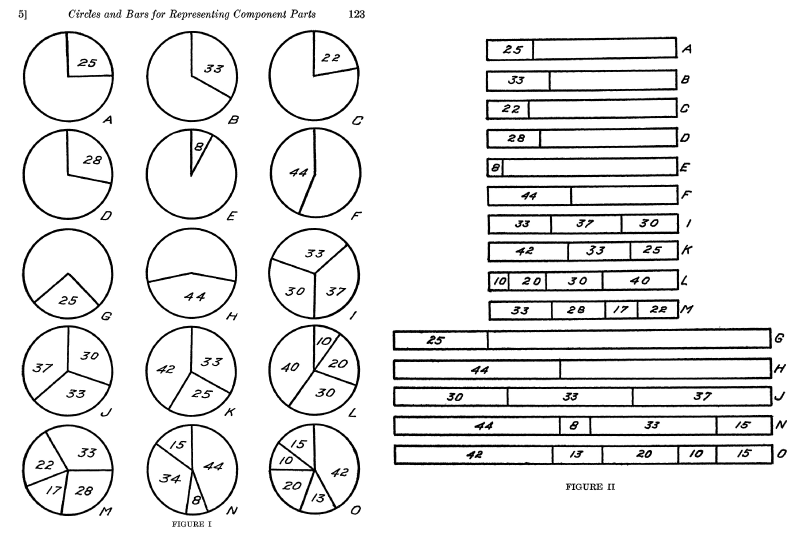
\includegraphics[height=0.45\textheight]{images/eells_experiment}    
  \end{center}
\end{frame}
